\documentclass[../main.tex]{subfiles}

%preamble
% \usepackage[subpreambles=true]{standalone}
% \usepackage{import}
% \usepackage{amsmath}%insert math equation
% \usepackage{graphicx} %insert picture
% \usepackage{subcaption}%insert pictures at the same place
% \usepackage{hyperref}%hyperlink
% \usepackage[a4paper]{geometry}
% \usepackage[section]{placeins}

% \title{Geometrical optics}
% \date{2018-02-04}
% \author{Hongjie Lu}

\begin{document}

	% \maketitle
	% \pagenumbering{gobble}
	% \newpage
	\section{Fermat's principle}

	Fermat's principle states that "light travels between two points along the path that requires the least time, as compared to other nearby paths." Thus it is mostly called "Fermat’s principle of least time".

	A more accurate statement of Fermat's principle: Any hypothetical small change in the actual path of a light ray would only result in a second order change in the optical path length. The first order change in the optical path length would be zero.

	\subsection{Reflection}
	\begin{figure}[h!]
		\centering
		\begin{subfigure}[b]{0.4\linewidth}
			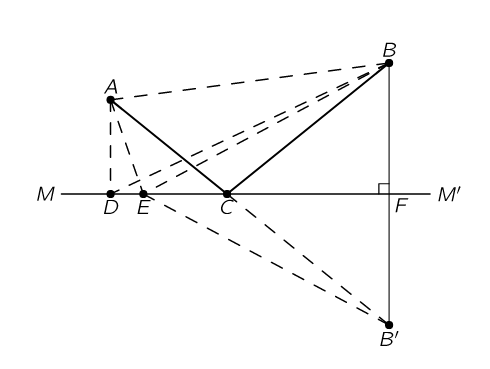
\includegraphics[width=\linewidth]{../graphics/Geometrical_optics1.png}
			% \caption{Illustration of Fermat’s principle for reflection}
		\end{subfigure}
		\begin{subfigure}[b]{0.4\linewidth}
			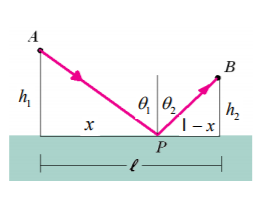
\includegraphics[width=\linewidth]{../graphics/Geometrical_optics2.png}
			% \caption{Relative shapes of conic surfaces in two dimensions}
		\end{subfigure}
		\caption{Illustration of Fermat’s principle for reflection}
	  	\label{fig:Fermat1}	  
	\end{figure}
	We can get the optical path length from the reflection case that:
	\begin{equation}
		L = \sqrt{x^2+h_1^2}+\sqrt{(l-x)^2+h_2^2}
	\end{equation}
	To minimize the optical path length or travel time we set the dericative of the equation with respect to x equal to zero.
	\begin{align}
		&\frac{dL}{dx}=\frac{x}{\sqrt{x^2+h^2}}+\frac{-(l-x)}{\sqrt{(l-x)^2+h_2^2}}=0\\
		&\frac{x}{\sqrt{x^2+h^2}}=\frac{(l-x)}{\sqrt{(l-x)^2+h_2^2}}\\
		&sin\theta_1=sin\theta_2\\
		&\theta_1=\theta_2
	\end{align}

	\subsection{Refraction}
	\begin{figure}[h!]
		\centering
		\begin{subfigure}[b]{0.4\linewidth}
			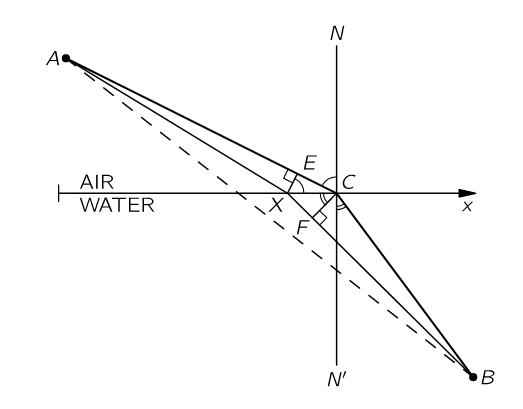
\includegraphics[width=\linewidth]{../graphics/Geometrical_optics3.png}
			% \caption{Illustration of Fermat’s principle for reflection}
		\end{subfigure}
		\begin{subfigure}[b]{0.4\linewidth}
			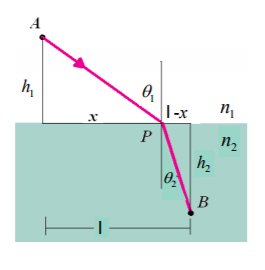
\includegraphics[width=\linewidth]{../graphics/Geometrical_optics4.png}
			% \caption{Relative shapes of conic surfaces in two dimensions}
		\end{subfigure}
		\caption{Illustration of Fermat’s principle for refraction}
	  	\label{fig:Fermat1}	  
	\end{figure}
	Now we consider a light ray traveling from point A to point B in media with different indices of refraction. The optical path length, which is also proportional to the travel time, between the two points is the product of the geometric length of the path and the index of refraction of the medium.
	\begin{equation}
		L = n_1\sqrt{x^2+h_1^2}+n_2\sqrt{(l-x)^2+h_2^2}
	\end{equation}
	To minimize the optical path length we set the dericative of the equation with respect to x equal to zero.
	\begin{align}
		&\frac{dL}{dx}=n_1\frac{x}{\sqrt{x^2+h^2}}+n_2\frac{-(l-x)}{\sqrt{(l-x)^2+h_2^2}}=0\\
		&n_1\frac{x}{\sqrt{x^2+h^2}}=n_2\frac{(l-x)}{\sqrt{(l-x)^2+h_2^2}}\\
		&n_1sin\theta_1=n_2sin\theta_2
	\end{align} 
	which is Snell's law
	\section{Paraxial optics}
	\subsection{Single spherical surface}
	\begin{figure}[h!]
		\centering
		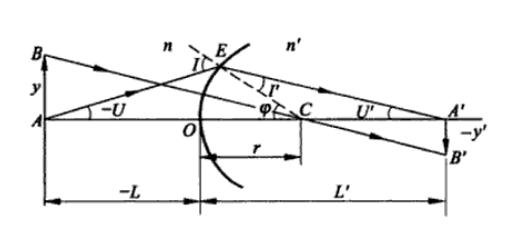
\includegraphics[scale=0.7]{../graphics/Geometrical_optics5.png}
		\caption{Single spherical surface}
		\label{fig:spherical}
	\end{figure}
	From the figure, we can have:
	\begin{align}
		&\frac{sin(-U)}{r}=\frac{sin(I)}{r-L}\\
		&\Rightarrow sinI=\frac{L-r}{r}sinU\label{eq:1}\\
		&n'sinI'=nsinI\label{eq:2}\\
		&\varphi=I+U=I'+U'\\
		&\Rightarrow U'=I+U-I'\\
		&\frac{sinU'}{r}=\frac{sinI'}{L'-r}\label{eq:3}\\
		&\Rightarrow L'=r+r\frac{sinI'}{sinU'}
	\end{align}
	$U$ and $L$ are the function of $U'$ and $L'$, so we can get $U'$ and $L'$ when provided $U$ and $L$. The specific rays from object point with fixed $U$ and $L$ will get the image point with the same $U'$ and $L'$, but one object point normally can have different angles of $U$, which means the image through the spherical refractive surface will not focus at one point, as shown in the figure.
	\begin{figure}[h!]
		\centering
		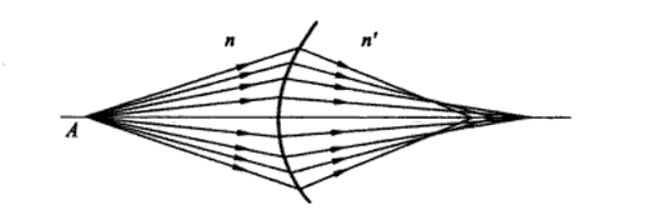
\includegraphics[scale=0.7]{../graphics/Geometrical_optics6.png}
		\caption{Non-perfect imaging of single spherical surface}
		\label{fig:imperfection}
	\end{figure}
	
	\subsubsection{Paraxial approximation}
	If we confine the rays in a small angle to axis, which means the value of angle $U$, $I$, $U'$, and $I'$ is small, here replaced by $u$, $i$, $u'$, and $i'$ respectively. And $L$ and $L'$ are replaced by $l$ and $l'$. So we can get following equations when we approcimate the angle sin value with its arc value:
	\begin{align}
		&\frac{-u}{r}=\frac{i}{r-l}\\
		&\Rightarrow i=\frac{L-r}{r}u\\
		&n'i'=ni\\
		&\varphi=i+u=i'+u'\\
		&\Rightarrow u'=i+u-i'\\
		&\frac{u'}{r}=\frac{i'}{l'-r}\\
		&\Rightarrow l'=r+r\frac{i'}{u'}
	\end{align}
	We can derive that $l'=\frac{n'l}{n'l-n(l-r)}$, $l'$ is independent with the angle $u$, which means the paraxial rays of one object point can perfectly form a image point.
	Another form of the last equation is:
	\begin{equation}
		\frac{n'}{l'}-\frac{n}{l}=\frac{n'-n}{r}=\varphi
	\end{equation}
	We call $\varphi$ the focal power of the specific medium and surface, which indicates the degree of optical system converging or diverging light. The SI unit for optical power is the inverse metre($m^{-1}$).
	or in form of:
	\begin{equation}
		n'\left(\frac{1}{r}-\frac{1}{l'}\right)=n\left(\frac{1}{r}-\frac{1}{l}\right)=Q
	\end{equation}
	Q is called the Abbe Invariant.\\
	\begin{figure}[h!]
		\centering
		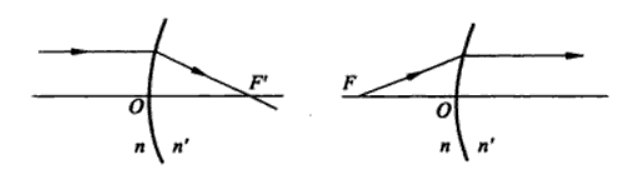
\includegraphics[scale=0.7]{../graphics/Geometrical_optics7.png}
		\caption{Object/Image at infinite distance}
		\label{fig:infinite}
	\end{figure}\\
	If the object is at infinite distance, $l\to-\infty$
	\begin{equation}
		l_{l=-\infty}'=f'=\frac{n'}{n'-n}r
	\end{equation}
	Similiarly, if the image is at infinite distance, $l'\to\infty$
	\begin{equation}
		l_{l'=-\infty}=f=-\frac{n}{n'-n}r
	\end{equation}
	\begin{align}
		&f+f'=r\\
		&\varphi=\frac{n'}{f'}=-\frac{n}{f}\\
		&\frac{f'}{f}=-\frac{n'}{n}
	\end{align}
	\subsubsection{Transverse magnification}
	\begin{figure}[h!]
		\centering
		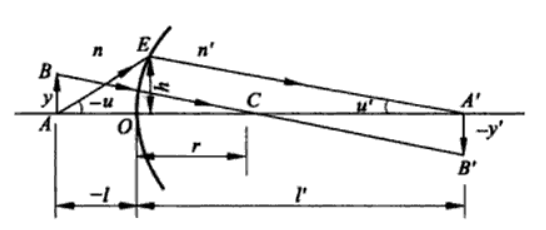
\includegraphics[scale=0.5]{../graphics/Geometrical_optics8.png}
		\caption{Transverse magnification}
		\label{fig:transverse}
	\end{figure}
	\FloatBarrier
	Transerve magnification is the height of the image divided by that of object.
	\begin{align}
	&\beta=\frac{y'}{y}\\
	&\frac{-y'}{y}=\frac{l'-r}{-l+r}\\
	&\Rightarrow\frac{y'}{y}=\frac{l'-r}{l-r}\\
	&\beta=\frac{y'}{y}=\frac{nl'}{n'l}(based\ on\ equation\ before)
	\end{align}
	\subsubsection{Longitude magnification}
	Longitude magnification is the relation between displacements of a pair of conjugate points. Longitude magnification $\alpha$ is the object axial displacement divided by the image axial displacement.
	\begin{equation}
		\alpha=\frac{dl'}{dl}
	\end{equation}
	from former equation $\frac{n'}{l'}-\frac{n}{l}=\frac{n'-n}{r}$, we take the derivative and get,
	\begin{align}
		&-\frac{n'dl'}{{l'}^2}+\frac{ndl}{l^2}=0\\
		&\alpha=\frac{dl'}{dl}=\frac{nl'^2}{n'l^2}=\frac{n'}{n}\beta^2
	\end{align}
	We can see the longitude magnification is always positive, which means the image moves in the same direction as object moves. This equation is only applible for the adjacence of the point. Similarly, we can derive the longitude magnification for two axial object point,
	\begin{figure}[h!]
		\centering
		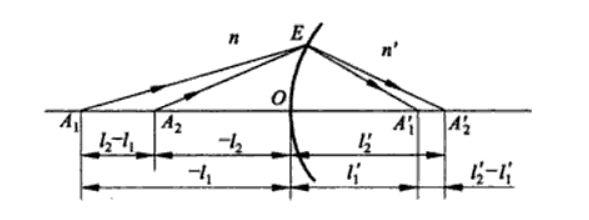
\includegraphics[scale=0.5]{../graphics/Geometrical_optics9.png}
		\caption{Longitude magnification}
		\label{fig:longitude}
	\end{figure}
	\begin{equation}
		\alpha=\frac{l_2'-l_1'}{l_2-l_1}=\frac{n'}{n}\beta_1\beta_2
	\end{equation}
	\subsubsection{Angular magnification}
	Angular magnification is defined as the ratio of angles between conjugate paraxial rays and optical axis.
	\begin{align}
	&\gamma=\frac{u'}{u}\\
	&for\ paraxial\ case,\ lu=l'u',\ then,\\
	&\gamma=\frac{l}{l'}=\frac{n}{n'}\frac{1}{\beta}
	\end{align}
	\subsubsection{Relation among magnifications}
	From above, the relation among three magnifications shows $\alpha\gamma=\beta$
	\subsubsection{Lagrange-Helmoltz invariant}
	From $\beta=\frac{y'}{y}=\frac{nl'}{n'l}$ and $lu=l'u'$, we can get the Lagrange-Helmoltz invariant $J=nuy=n'u'y'$. It is the production of object height, aperture angle and medium index.
	\subsection{Reflective spherical mirror}
	\begin{figure}[h!]
		\centering
		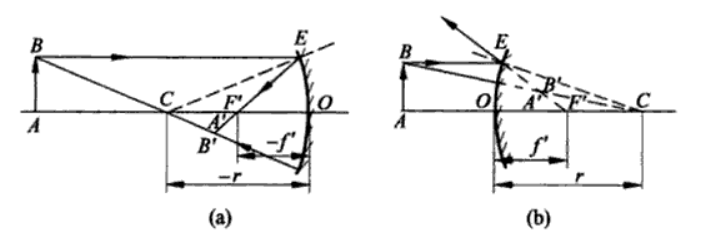
\includegraphics[scale=0.5]{../graphics/Geometrical_optics10.png}
		\caption{Reflective spherical mirror}
		\label{fig:Reflective}
	\end{figure}
	Similarly, for reflective spherical lens, we can make $n'=-n$, and will get corresponding equations.
	\begin{equation}
		\frac{1}{l'}+\frac{1}{l}=\frac{2}{r}
	\end{equation}
	for infinite image or object
	\begin{equation}
		f'=f=\frac{r}{2}
	\end{equation}
	and for the magnifications,
	\begin{align}
		&\beta=\frac{y'}{y}=\frac{nl'}{n'l}=-\frac{l'}{l}\\
		&\alpha=\frac{n'}{n}\beta^2=-\beta^2\\
		&\gamma=\frac{n}{n'}\frac{1}{\beta}=-\frac{1}{\beta}
	\end{align}
	\subsection{Thin lens}
	A thin lens is a lens with a thickness(distance along the optical axis between the two surfaces of the lens) that is negligible compared to the radii of curvature of the lens surfaces.
	The thin lens approximation ignores optical rffects due to the thickness of lenses and simplifies ray tracing calculations. It is often combined with the paraxial approximation in techiques such as ray transfer matrix analysis.
	The assumptions for thin lens are $n_1=n_2'=1$(air), $n_1'=n_2=n$(lens index)
	\begin{align}
		&n\left(\frac{1}{r_1}-\frac{1}{l_1'}\right)=1*\left(\frac{1}{r_1}-\frac{1}{l_1}\right)\\
		&n\left(\frac{1}{r_2}-\frac{1}{l_2'}\right)=1*\left(\frac{1}{r_2}-\frac{1}{l_2}\right)\\
		&l_2=l_1'\\
		&\Rightarrow(n-1)\left(\frac{1}{r_1}-\frac{1}{r_2}\right)=\frac{1}{l'}-\frac{1}{l}
	\end{align}
	\begin{figure}[h!]
		\centering
		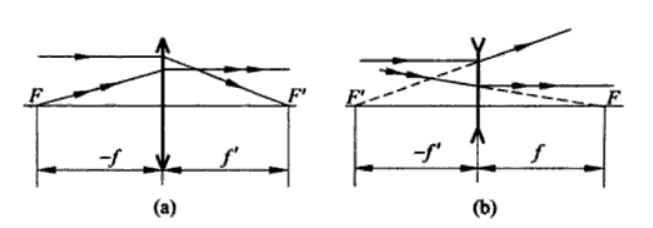
\includegraphics[scale=0.8]{../graphics/Geometrical_optics11.png}
		\caption{Convex and concave}
		\label{fig:lens}
	\end{figure}
	For infinite object or image, we can get the focus length,
	\begin{align}
		&f'=-f=\frac{1}{(n-1)\left(\frac{1}{r_1}-\frac{1}{r_2}\right)}\\
		&\varphi=\varphi_1+\varphi_2=\frac{1}{f'}=(n-1)\left(\frac{1}{r_1}-\frac{1}{r_2}\right)\\
		&\frac{1}{l'}-\frac{1}{l}=\frac{1}{f'}
	\end{align}
	\subsection{Cardinal points}
	Gaussian optics(paraxial ray-tracing), or coaxial ideal optical system, normally extends the results of the paraxial approximation.\\
	In Gaussian optics, the cardinal points consist of three pairs of points located on the optical axis of a rotationally symmetric, focal, optical system. These are the focal points, the principal points, and the nodal points. For ideal systems, the basic imaging properties such as image size, location, and orientation are completely determined by the locations of the cardinal points; in fact only four points are necessary: the focal points and either the principal or nodal points. The only ideal system that has been achieved in practice is the plane mirror, however the cardinal points are widely used to approximate the behavior of real optical systems. Cardinal points provide a way to analytically simplify a system with many components, allowing the imaging characteristics of the system to be approximately determined with simple calculations.\\
	By definition, the image focus $F'$ of an optical system is the image of the infinite point on the axis. The beam issued out of this point is made of parallel rays to the axis.\\
	These rays focalise in $F'$ after crossing the system. The location of the intersection points of each incident ray with its corresponding image ray is, in paraxial approximation, a plane which shall be called image principal plane of the optical system.\\
	This plane cuts the axis in $H'$, $f'=H'F'$ is the focal image distance of the optical system. $H'$ is the image principal point. We proceed in the same way as for the object focus $F$, the object principal plane, the object focal distance $f=HF$.

	\begin{figure}[h!]
		\centering
		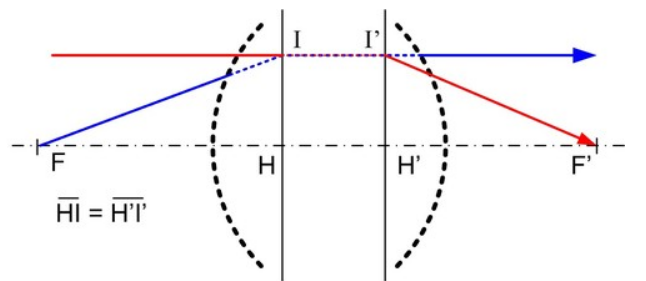
\includegraphics[scale=0.8]{../graphics/Geometrical_optics12.png}
		\caption{Cardinal points}
		\label{fig:Cardinal}
	\end{figure}
	\FloatBarrier
	Any luminous ray issued from $F$ cust the object principal plane in $I$ and comes out parallel to the axis, it cuts the image principal plane in $I'$. An incident ray parallel to the axis groing through $I$, also goes through $I'$ the converges in $F'$. These two rays cross each other in $I$ in the object space then in $I'$ in the image space $I$ and $I'$ are therefore conjugated.\\
	The principal planes are conjugated with an associated transversal magnification equal to 1.\\
	\textbf{Nodal points}\\
	\begin{figure}[h!]
		\centering
		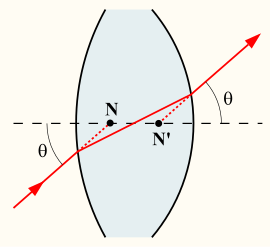
\includegraphics[scale=0.8]{../graphics/Geometrical_optics16.png}
		\caption{Nodal points}
		\label{fig:Nodal points}
	\end{figure}
	\FloatBarrier
	The front and rear nodal points have the property that a ray aimed at one of them will be refracted by the lens such that it appears to have come from the other, and with the same angle with respect to the optical axis. \\
	If the medium on both sides of the optical system is the same (e.g., air), then the front and rear nodal points coincide with the front and rear principal points, respectively.
	\subsection{Marginal and Chief Rays}
	the ray that passes from the center of the object, at the maximum aperture of the lens, is normally known as the marginal ray. It therefore passes through the edge of the aperture stop. Conventionally, this ray is in the y-z plane, usually called the meridian plane.

	The chief ray is defined to be the ray from an off-axis point in the object passing through the center of the aperture stop; although there can be an infinite number of such rays, we can usually assume, at least for centered systems, that the chief ray is also restricted to the meridian plane.
	\begin{figure}[h!]
		\centering
		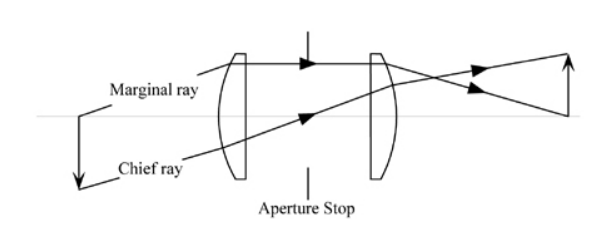
\includegraphics[scale=0.8]{../graphics/Geometrical_optics13.png}
		\caption{Simple lens system and aperture stop.}
		\label{fig:ray}
	\end{figure}
	\subsection{Reference}
	\url{https://books.google.de/books?id=vI7-WDw7yxkC&printsec=frontcover#v=onepage&q&f=false}

	\section{Aberration}
	The optic design based on paraxial approximation owns small numerical aperture and small field angle. The need for an aberration theory valid for more complicated optical systems with larger values of numerical aperture and field angle was felt when photography emerged.\\
	Aberration can be defined as a departure of the performance of an optical system from the predictions of paraxial optics.\\
	The Five Seidel Aberrations\\
	The five basic types of aberration which are due to the geometry of lenses or mirrors, and which are applicable to systems dealing with monochromatic light, are known as Seidel aberrations, from an 1857 paper by Ludwig von Seidel. These are the aberrations that become evident in third-order optics, also known as Seidel optics.
	As we know,

	\begin{align}
		&sinx=x-\frac{x^3}{3!}+\frac{x^5}{5!}-\frac{x^7}{7!}+\frac{x^9}{9!}-\frac{x^11}{11!}+\frac{x^13}{13!}-...\\
		&cosx=1-\frac{x^2}{2!}+\frac{x^4}{4!}-\frac{x^6}{6!}+\frac{x^8}{8!}-\frac{x^10}{10!}+\frac{x^12}{12!}-...
	\end{align}

	When we neglect the later terms in the series, so that we behave as if $sin(x) = x$, and $cos(x) = 1$, we obtain first-order optics, in which all lenses are perfect. When we include the $x$ squared and $x$ cubed terms, then we have proceeded to third-order optics, in which the aberrations resulting from the nature of real lenses, exclusive of chromatic aberration, become evident.
	The five Seidel aberrations are:
	\subsection{Spherical Aberration}
	this is the aberration affecting rays from a point on the optical axis; because rays from this point going out in different directions pass through different parts of the lens, then, if the lens is spherical, or otherwise not the exact shape needed to bring them all to a focus, then these rays will not all be focused at the same point on the other side of the lens.
	\subsection{Coma}
	this aberration affects rays from points off the optical axis. If spherical aberration is eliminated, different parts of the lens bring rays from the axis to the same focus. But the place where the image of an off-axis point is formed may still change when different parts of the lens are considered.
	\subsection{Astigmatism}
	this is another aberration affecting rays from a point off the optical axis. These rays, as they head through the lens to the point in the image where they will be focused, pass through a lens that is, from their perspective, tilted. Even if neither spherical aberration nor coma prevents them from coming to a sharp focus, if we consider the rays of light that are in the plane of the tilt, and the rays of light that are in the plane perpendicular to that, these rays pass through a part of the lens with a different profile. So they may not be focused at the same distance from the lens, even if they do come to a focus in each case.
	\subsection{Curvature of Field}
	even when light from every point in the object is brought to a sharp focus, the points at which they are brought into focus might lie on a curved surface instead of a flat plane.
	\subsection{Distortion}
	even when all the previous aberrations have been corrected, the light from points in the object might be brought together on the image plane at the wrong distance from the optical axis, instead of being linearly proportional to the distance from the optical axis in the object. If distance increases faster than in the object, one has pincushion distortion, if more slowly, barrel distortion.
	\begin{figure}[h!]
		\centering
		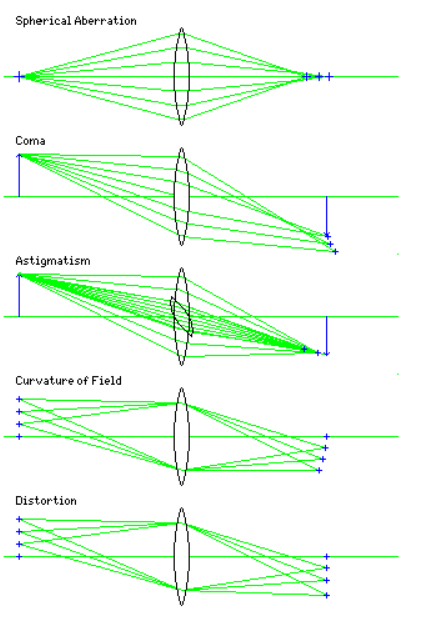
\includegraphics[scale=0.8]{../graphics/Geometrical_optics14.png}
		\caption{Seidel Aberrations}
		\label{fig:Aberration}
	\end{figure}
	\subsection{Reference}
	\url{http://www.quadibloc.com/science/opt0505.htm}

	\subsection{Abbe sine condition}
	From equations \ref{eq:1} \ref{eq:2} \ref{eq:3} above we can also get the abbe sine condition, using $\frac{AB}{AC}=\frac{A'B'}{A'C}$, then $nysinU=n'y'sinU'$\\
	We can also derive the Abbe sine condition by eikonal equation.
	\begin{figure}[h!]
		\centering
		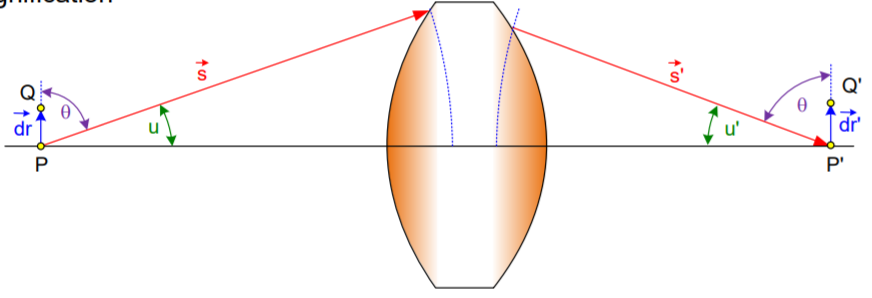
\includegraphics[scale=0.7]{../graphics/Geometrical_optics15.png}
		\caption{eikonal equation}
		\label{fig:eikonal}
	\end{figure}
	\begin{align}
		&\delta L=n'\vec{s'}d\vec{r'}-n\vec{s}d\vec{r}=0\\
		&n'\vec{s'}d\vec{r'}=n\vec{s}d\vec{r}\\
		&n'd\vec{r'}cos\theta'=nd\vec{r}cos\theta\\
		&nsin\varphi=n'\beta sin\varphi'
	\end{align}

	\section{Index}
	Taylor series:
	$sinx=x-\frac{x^3}{3!}+\frac{x^5}{5!}-...$\\
	$\sqrt{1-x^2}=1-\frac{x^2}{2}-\frac{x^4}{8}-...$\\
	numerical aperture v.s. f-number, written f/ or N\\
	$NA=nsin\theta$\\
	$N=\frac{f}{D}$\\
\end{document}